% tesi.tex
%
% thesis (c) by Franco Masotti <franco.masotti@student.unife.it>
%
% thesis is licensed under a
% Creative Commons Attribution-ShareAlike 4.0 International License.
%
% You should have received a copy of the license along with this
% work. If not, see <http://creativecommons.org/licenses/by-sa/4.0/>.
%

\documentclass[10pt,titlepage,twoside,a4paper]{report}
\usepackage[backend=biber]{biblatex}
\addbibresource{ref.bib}
\usepackage{mathtools}
\usepackage[margin=1in,a4paper]{geometry}
\usepackage[italian]{babel}
\usepackage{lmodern}
\usepackage[utf8]{inputenc}
\usepackage{graphicx,url,amsfonts,epsfig,hyperref,float,listings}
%\usepackage{float}
%\floatstyle{boxed} 
%\restylefloat{figure}
\usepackage{caption}
\usepackage{minted}
\usepackage[usenames,dvipsnames,svgnames,table]{xcolor}
\usepackage{tikz}
\usepackage{csquotes}
\renewcommand{\mkbegdispquote}[2]{\itshape}
\usepackage{setspace}
    \doublespacing
\DeclareCaptionFont{white}{\color{white}}
\DeclareCaptionFormat{listing}{\colorbox{gray}{\parbox{\textwidth}{#1#2#3}}}
\captionsetup[listing]{justification=centering,format=listing,labelfont=white,textfont=white}
\DeclareCaptionFormat{figure}{\colorbox{gray}{\parbox{\textwidth}{#1#2#3}}}
\captionsetup[figure]{justification=centering,format=listing,labelfont=white,textfont=white}

\newenvironment{code}{\singlespacing\captionsetup{type=listing}}{}

% Manually change the language otherwise it does not work.
\renewcommand{\listingscaption}{Listato}
\renewcommand{\listoflistingscaption}{Elenco dei listati}

%%%%%% Enable to debug
%\usepackage{showframe}

\definecolor{bg}{rgb}{0.95,0.95,0.95}

% Global minted options.
\usemintedstyle{tango}
% Verbatim imput
\newminted{text}{fontsize=\footnotesize,frame=single,framesep=10pt,breaklines,bgcolor=bg,linenos=true}
\newminted{prolog}{fontsize=\footnotesize,frame=single,framesep=10pt,breaklines,bgcolor=bg,linenos=true}
\newminted{r}{fontsize=\footnotesize,frame=single,framesep=10pt,breaklines,bgcolor=bg,linenos=true}
\newminted{shell}{fontsize=\footnotesize,frame=single,framesep=10pt,breaklines,bgcolor=bg,linenos=true}

% Inputfiles
\newmintedfile[bashcodefile]{bash}{fontsize=\footnotesize,frame=single,framesep=10pt,breaklines,bgcolor=bg,linenos=true}
\newmintedfile[prologcodefile]{prolog}{fontsize=\footnotesize,frame=single,framesep=10pt,breaklines,bgcolor=bg,linenos=true}


%%%%
%%%%
%%%%
%%%%


\title{Integrazione di una applicazione web con strumenti per la statistica}
%\title{\textsc{Integrazione di una applicazione web con strumenti per la statistica}}
\author{Franco Masotti}

\begin{document}
\pagenumbering{roman}

\maketitle
\newpage
\tableofcontents
\newpage
\listoffigures
\newpage
%\listoftables
%\newpage
\listoflistings
\cleardoublepage

\pagenumbering{arabic}


%%%%
%%%%
%%%%
%%%%


\chapter{Introduzione}
\label{introduzione}

[TODO]

\chapter{Specifiche del problema}
\label{ch:specifiche-del-problema}
    \section{Componenti software}
Per spiegare il problema è necessario introdurre i software principali che si 
sono utilizzati.

La piattaforma \emph{SWISH}\cite{swish} viene usata per la programmazione 
logica attraverso un qualunque web browser dotato di \emph{Javascript}. Questa 
è collegata direttamente all'interprete SWI.

\emph{Cplint on SWISH} è una versione modificata di SWISH che include la 
libreria \emph{cplint}, la quale permette di formulare inferenze 
probabilistiche e compiere processi di apprendimento\cite{cplint}.

\emph{R} è un ambiente software dedicato alla statistica e 
alla rappresentazione grafica di dati\cite{r}.

\emph{SWI Prolog} è un interprete per la programmazione 
logica\cite{swiprolog}, come suggerisce il nome\cite{prolog}.

    \section{Obbiettivi}
L'obbiettivo di questa tesi è quello di illustrare come 
permettere alla libreria Cplint on SWISH di usare R.
Si spiegherà infine come si è semplificata l'installazione di questo ambiente 
software.

        \subsection{Funzioni grafiche}
SWISH offre due tipi di funzionalità grafiche, una attraverso C3.js e l'altra
attraverso R. C3.js è una libreria Javascript che a sua volta deriva da
D3.js, acnhe chiamata \emph{Data-Driven Documents}. Anche in questo caso si 
tratta di una libreria grafica Javascript che permette di visualizzare
dei dati utilizzando la Scalable Vector Graphics (\emph{SVG}), l'elemento 
\emph{Canvas}, un'area all'interno di un pagina web nella quale è possibile 
disegnare in due dimensioni\cite{canvasHtml}, e il linuguaggio 
HTML\cite{d3js}. Questi grafici, inoltre, sono interattivi a differenza di 
quelli di quelli generabili da R.

Il package R \emph{ggplot2} 
permette di disegnare gafici usando la 
cosiddetta \emph{grammatica dei grafici}, cioè la divisione per contesti dei 
vari aspetti di un grafico come per esempio la geometria, la scala, la 
rappresentazione estetica, ed altri aspetti \cite{ggplot2OriginalDefinition}:
%% \cite{grammarOfGraphics} e 
%%\cite{ggplot2} e \cite{ggplot2OriginalDefinition}
%%[Sembra che la citazione originale sia stata rimossa dal sito ufficiale
%%di ggplot2.]

\begin{displayquote}
ggplot2 è un sistema di plotting per R, basato sulla grammatica dei grafici,
che cerca di utilizzare le parti migliori dei grafici di base e lattice, e di 
escludere le parti peggiori. Questo sistema si occupa della maggior parte dei
dettagli poco pratici che rendono il plotting problematico (come per esempio 
il disegno di legende), oltre che fornire un potente modello di grafica che
rende semplice produrre complessi plot con molteplici strati.
\end{displayquote}


        \subsection{Accesso ad R da Cplint on SWISH}
Nativamente Prolog non è in grado di accedere all'interprete R. Esistono 
tuttavia delle librerie che permettono di collegarsi all'interprete R
attraverso un \emph{socket} fornito da R stesso. Poiché stiamo utilizzando  
un \emph{server web}, per avere meno problemi di sicurezza, quali ad esempio 
\emph{privilege escalation}, il collegamento tra R e Prolog non può essere 
diretto ma avviene tramite un ambiente virtuale isolato chiamato Docker. 
Tutto questo però complica notevolmente l'installazione.


        \subsection{Semplificazione dell'installazione}
Per semplificare l'installazione e per renderla uniforme a quella di qualunque 
altro programma si sono creati alcuni \emph{pacchetti software} sia per 
le interfaccie web, sia per gli altri programmi descritti nelle sezioni 
precedenti.


%%%%
%%%%
%%%%
%%%%


\chapter{Strumenti e architettura}

%%
%%

    \section{R}
R è un ambiente software per il calcolo statistico e la 
visualizzazione grafica. Con il termine R si definisce 
l'interprete dei comandi mentre con S il linguaggio di programmazione. R 
comprende anche un gestore di pacchetti attraverso il quale si possono 
installare facilmente funzioni utili non comprese in R 
stesso \cite{rDefinition} ~\footnote{Da questo momento in poi, per semplicità, 
si userà il termine R per indicare anche il linguaggio.}

        \subsection{Comandi e operatori fondamentali}
Come la maggior parte dei linguaggi di programmazione, R mette a disposizione 
vari tipi di operatori tra cui quelli aritmetici, logici e di assegnazione.

Esistono varie possibilità per assegnare un valore ad una variabile. Di solito 
però viene preferita la notazione \mintinline{r}{<-} piuttosto che il classico 
\mintinline{r}{=}. Nel primo caso infatti non bisogna preoccuparsi di alcuni 
dettagli funzionali \cite{assignmentOperatorInR} \cite{rAssignmentOperator}

Una delle operazioni fondamentali di R è la funzione \mintinline{r}{c()}.
Questa serve per concatenare un insieme arbitrario di valori, in modo che 
questi possano essere salvati all'interno di un'unica variabile 
\cite{rVectorsAndAssignment} \cite{rConcatenatingLists}.

        \subsection{Oggetti}
R mette a disposizione strutture dati chiamate oggetti. Questi possono essere 
array di numeri, stringhe, funzioni, liste, \emph{data frame}, ed altre entità
\cite{rObject}.

In R le liste sono una collezione ordinata di oggetti, chiamati anche
componenti, che possono essere di tipo diverso tra di loro. Con le liste si 
ha la possibilità di accedere direttamente alle componenti sia attraverso il 
principio dell'indicizzazione, sia attraverso l'uso della notazione per nome,
del tipo \mintinline{r}{lista$componente}.
\cite{rList}

I \emph{data frame} sono un tipo particolare di oggetti che permettono 
di organizzare i dati sotto forma matriciale e sono definiti come 
specializzazione della classe lista \cite{rDataFrameDefinition}.  Rispetto ad 
una lista, infatti, esistono delle restrizioni tra le quali le più importanti
sono che le componenti devono essere vettori della stessa lunghezza 
\cite{rDataFrameRestrictions}. Un data frame può essere considerato per molti 
aspetti una matrice anche perchè si possono usare le stesse convenzioni per 
visualizzare e manipolare i dati \cite{rDataFrameSimilarToMatrices}. Tuttavia, 
a differenza delle matrici, i vettori che lo compongono possono avere valori
di tipo diverso, come avviene nelle tabelle \cite{rMatrices}.

Sia le liste sia i data frame verranno usati successivamente per gestire i 
dati.

%%
%%

\section{SWI Prolog e SWISH}
Prolog è un linguaggio di programmazione dichiarativo usato per 
esprimere relazioni tra elementi attraverso fatti e regole logiche 
\cite{prolog}.

SWI Prolog è una particolare implementazione del linguaggio Prolog. Si tratta 
di un ambiente di programmazione Prolog, libero e gratuito 
\cite{swiprolog}.

SWISH è un'interfaccia web di SWI Prolog \cite{swish}
ed ha lo scopo principale di far collaborare gli utenti per scrivere 
prolgrammi Prolog ed analizzarne i risultati.

%%
%%

\section{Cplint on SWISH}
Cplint è una suite di programmi di logica probabilistica. cplint comprende sia 
programmi per fare inferenze sia per l'apprendimento \cite{cplint} ed è 
incluso all'interno della versione di SWISH chiamata \emph{Cplint on SWISH} 
\cite{cplintOnSwish}.

%%%%
%%%%

    \section{rserve\_client}
rserve\_client è una libreria prolog che rende possibile 
l'accesso ad un ambiente R da parte di SWISH \cite{rserveClientDefinition} 
\cite{rserveclient}. Questa libreria include anche delle funzionalità per 
creare e gestire i data frame R direttamente da SWI Prolog 
\cite{swishRDataLibrary}.
    
        \subsection{Motivazione}
L'utilizzo di R rispetto a Prolog comporta in molti casi un netto miglioramento 
della velocità di calcolo \cite{rFaster}:
\begin{displayquote}
[..] È risultato che R è più veloce nel lavorare con una grande quantità
di numeri interi rispetto a Prolog. Perchè? Perchè una volta trasformato in R,
il vettore è un semplice array C di interi, e quindi molto veloce 
nell'addizione. La versione Prolog invece somma i numeri uno alla volta
oltre che controllare eventuali overflow.
\end{displayquote}

Un altro vantaggio nell'utilizzare R è la possibilità di accedere a tutte le 
funzionalità di computazione che non sono presenti in SWI Prolog, come ad 
esempio le funzioni per studi statistici.
 
\subsection{Scambiare dati fra R e Prolog}
Esistono due modalità per usare i comandi di R all'interno di SWI Prolog:
\begin{itemize}
    \item come \emph{Prolog term}, usando l'operatore \mintinline{r}{<-} 
seguito dal comando R,
    \item oppure con una notazione chiamata \emph{quasi-quotation}
\end{itemize}
La documentazione di SWISH contiene un esempio per entrambi i 
casi\cite{rprolognotations}:
\begin{displayquote}
- Le quasi quotations possono essere usate per fare copia incolla del codice R 
nel proprio programma Prolog senza necessità di cambiarlo (tranne quando 
contiene \texttt{|\}}).

- Il codice Prolog protrebbe aver bisogno di piccole modifiche. Nell'esempio,
  \mintinline{r}{I(.5)} deve essere cambiato in \mintinline{r}{'I'(0.5)} perchè 
  i floating point in prolog non possono iniziare con \texttt{.} e gli 
  argomenti (usati come simboli di funzioni) non possono iniziare con una lettera 
  maiuscola. L'utilizzo del prolog term tuttavia

    - È più compatibile.

    - Giova del controllo della sintassi Prolog.

    - Rende più facile comporre espressioni R da elementi più piccoli.
\end{displayquote}
Per l'esempio in Prolog term si veda il listato \ref{lst:esempioPrologTerm}
mentre per l'esempio quasi quotation si veda il 
listato \ref{lst:esempioquasiQuotation}.
Come si vede nel primo caso è necessario fare qualche piccola modifica 
rispetto all'originale R. Nel secondo caso invece è possibile gestire alcuni 
casi particolari che genererebbero errori oppure che non sarebbe possibile 
trasformare nel primo caso.

\begin{code}
    \caption{Esempio notazione Prolog term}
    \label{lst:esempioPrologTerm}
    \begin{prologcode*}{}
<- qplot(mpg, data=mtcars, geom="density", fill=gear, alpha='I'(0.5), main="Distribution of Gas Milage", xlab="Miles Per Gallon", ylab="Density").
    \end{prologcode*}
\end{code}

\begin{code}
    \caption{Esempio notazione quasi quotation}
    \label{lst:esempioquasiQuotation}
    \begin{prologcode*}{}
<- {|r||qplot(mpg, data=mtcars, geom="density", fill=gear, alpha=I(.5), main="Distribution of Gas Milage", xlab="Miles Per Gallon", ylab="Density")|}.
    \end{prologcode*}
\end{code}

%%%%
%%%%

\section{Rserve ed rserve-sandbox}

\emph{Rserve} è un server che permette ad altri programmi di
utilizzare gli strumenti messi a disposizione da R attraverso diversi
linguaggi di programmazione, senza dover inizializzare R o
linkarne la libreria \cite{rserve}. Rserve è il software attraverso il quale 
rserve\_client può interfacciarsi con R.

Per migliorare la sicurezza Rserve non 
viene mai eseguito direttamente, ma all'interno di un sistema di 
virtualizzazione chiamato Docker. Inoltre non viene mai esposto un socket 
\emph{TCP/IP} ma solo un socket di tipo \emph{UNIX}. A differenza di socket 
TCP/IP, in un socket UNIX tutto lo scambio di dati avviene all'interno del 
\emph{kernel} del sistema operativo \cite{unixSocket}. 
L'applicazione di quest'ultimo aspetto si può vedere nel 
listato~\ref{lst:rservconf} che contiene la configurazione di Rserve.

Le modalità di funzionamento di reserve-sandbox sono spiegate nello schema in 
figura~\ref{fig:rserveSandboxScheme}, 

\begin{figure}[H]
\centering
\caption{Schema funzionamento di rserve sandbox}
\begin{tikzpicture}
    \draw[thick] 
(-5,5) -- node[align=left, below]{Sistema}
(5,5) -- 
(5,-5) -- 
(-5,-5) --
cycle;
    \draw[thick]
(-4,3) -- node[align=left, below]{Istanza Docker}
(1,3) --
(1,-4) --
(-4, -4) --
cycle;
    \draw[thick]
(-2,-1) -- node[align=left, below]{Socket \\ UNIX \\ Rserve}
(0,-1) --
(0,-3) --
(-2, -3) --
cycle;
    \draw[thick]
(2,-1) -- node[align=left, below]{Processo \\ SWISH}
(4,-1) --
(4,-3) --
(2, -3) --
cycle;
    \draw[thick, red, ->]
(0,-1.5) --
(2,-1.5);
    \draw[thick, red, ->]
(2,-2.5) --
(0,-2.5);
\end{tikzpicture}
\label{fig:rserveSandboxScheme}
\end{figure}

\begin{code}
    \caption{File di configurazione di Rserve}
    \bashcodefile{Rserv.conf}
    \label{lst:rservconf}
\end{code}

%%%%
%%%%

    \section{Docker}
\emph{Docker} è un implementazione di una virtualizzazione a 
livello di sistema operativo, cioé permette l'esistenza di molteplici istanze 
di ambienti isolati basate su utenti separati. Con Docker, in particolare, 
questi ambienti possono essere eseguiti su una qualunque macchina in modo 
indipendente dalla configurazione del sistema operativo e sono eseguiti dal 
singolo kernel del sistema operativo ospite. In questo modo il software che è 
eseguito al loro interno è garantito funzionare in modo affidabile e come lo 
sviluppatore aveva inteso che funzionasse
\cite{operatingSystemLevelVirtualization} \cite{docker}.

        \subsection{Immagini}
Attraverso un documento di testo chiamato \emph{Dockerfile}, Docker viene 
usato per costruire un'\emph{immagine} che comprende un'insieme di 
programmi, file, utenti e tutto ciò che è necessario allo svolgimento di
un specifico compito. Le istruzoni nel documento di testo sono nella forma
\mintinline{bash}{ISTRUZIONE_DOCKER argomento}. Per aggiungere utenti, 
gruppi ed altre operazioni viene usata l'istruzione \textbf{RUN} seguita dal 
percorso di una shell disponibile e infine dal comando che deve essere eseguito. Per 
semplicità si può anche omettere la shell ne verrà usata una di default. Per 
esempio
\mint{bash}|RUN /bin/bash -c groupadd -g newgroupid groupname|

Altri comandi importanti sono:
\begin{itemize}
    \item \textbf{CMD}: stabilisce l'istruzione che deve essere 
eseguita ad ogni avvio dell'immagine
    \item \textbf{ENV}: imposta variabili d'ambiente
    \item \textbf{USER}: effettua un cambio di utente per tutti i comandi che lo seguono
    \item \textbf{WORKDIR}: cambia directory
    \item \textbf{ADD}: copia file nell'immagine
\end{itemize}

Dopo aver costruito l'immagine con \mint{bash}|docker build <nome 
immagine> .|
la si può eseguire con \mint{bash}|docker run <nome immagine>|
L'istanza di un immagine è chiamata \emph{container} 
\cite{DockerfileReference}.

Utilizzando i dockerfile la comunità di utilizzatori di Docker continua a 
creare e a distribuire nuove immagini precomilate ognuna con un particolare 
utilizzo.
Il vantaggio di questo metodo è che l'utente finale è in grado di utilizzare 
subito l'immagine, senza che possano sorgere problemi nella fase di build. Lo 
svantaggio tuttavia è che l'immagine può  essere anche molto grande 
(nell'ordine del Gigabyte) e quindi difficile da distribuire con i mezzi di 
rete più noti.

    \subsection{Configurazioni di Docker per utilizzare rserve-sandbox}
Per l'utilizzo dell'ambiente R all'interno di rserve-sandbox è necessario che 
Rserve sia integrato opportunamente con Docker. Il \emph{Dockerfile} che si 
è utilizzato contiene infatti le instruzioni per installare e avviare Rserve.
La seguente istruzione consente di installare il pacchetto R ggplot2.

\begin{code}
    \caption{Istruzione installazione pacchetto R}
    \begin{shellcode*}{}
RUN echo 'install.packages(c("ggplot2"), repos="http://cloud.r-project.org/", dependencies=TRUE)' > /tmp/packages.R \
    && Rscript /tmp/packages.R
    \end{shellcode*}
\end{code}

Con il comando \mintinline{bash}{CMD /bin/bash Rserv.sh}, presente nel 
Dockerfile,
Docker chiama Rserve con la configurazione presente nel 
listato~\ref{lst:rservconf} presente a pagina~\pageref{lst:rservconf}.

Dopo aver generato l'immagine si può avviare il container.
Le opzioni che serve passare al comando \texttt{docker} sono:
\begin{itemize}
    \item  \texttt{--net=none}, in quanto non ci serve uno stack di rete
    \item  \texttt{--rm}, perchè non ci interessa salvare il container per
           un futuro utilizzo. Infatti ogni volta ne verrà creato uno nuovo.
           Senza questa opzione la memoria di massa si riempirebbe dopo
           vari avvii.
    \item  \texttt{-v /home/rserve:/home/rserve}, che serve a montare 
           la directory /home/rserve del sistema host in quello guest.
           In questa directory sarà infatti presente il socket di Rserve,
           in modo da essere accessibile al daemon di SWISH.
\end{itemize}
Nel listato~\ref{lst:dockerruncommand} si trova il comando completo.

\begin{code}
    \caption{Comando per avviare il container}
    \begin{shellcode*}{}
docker run --net=none --rm -v /home/rserve:/home/rserve rserve
    \end{shellcode*}
    \label{lst:dockerruncommand}
\end{code}

%%%%
%%%%

\section{QVM}
Per completare tutto il lavoro e testare le modifiche sui programmi man 
mano, è stato necessario installare l'intera piattaforma sul computer. 
Questo è stato possibile attraverso l'utilizzo di macchine virtuali 
per ragioni di comodità.

\subsection{Macchine virtuali}
Per agevolare l'installazione ed il mantenimento della piattaforma web su una 
istanza locale si sono utilizzate macchine virtuali con immagini di 
distribuzioni GNU/Linux diverse quali: Antergos, Parabola GNU/Linux-libre, 
Debian e Trisquel.

\subsubsection{Qemu Virtual Machine}
Utilizzando il programma \emph{QEMU} \cite{qemu} si è potuto scrivere uno
script shell, \emph{QVM}, in modo da gestire facilmente tutti i casi d'uso che 
si sono presentati \cite{qvm}. Questo si è rivelato molto utile per esempio per 
gestire i backup dei dischi rigidi virtuali. Infatti per testare nuovi 
pacchetti e programmi è consigliabile partire sempre da un sistema pulito
per evitare che precedenti installazioni possano alterare il funzionamento.
Con QVM sono infatti sufficienti un paio di comandi per ripristinare il 
backup e corregere l'errore.

Lo script dà anche la possibilità di condividere file fra la macchina host 
e guest attraverso una semplice directory.

Poiché l'interfaccia web di SWISH è accessibile attraverso un \emph{port} 
ben definito (di default \emph{3050}), si è fatto in modo che tale port 
fosse accessibile dalla macchina host con il port \emph{5555}. Infatti, a meno 
che non venga fatto un \emph{bridge} di rete la macchina virtuale ed il 
computer che la ospita lavorano su due sottoreti diverse. Bisogna quindi fare
un \emph{port forwarding} esplicito delle porte interessate.

Uno schema della relazione fra la macchina virtuale e l'host è disponibile 
nella figura~\ref{fig:schemaPortsQvm}.

\begin{figure}[H]
\centering
\caption{Schema della relazione tra i port della macchina host e guest}
\label{fig:schemaPortsQvm}
\begin{tikzpicture}
    \draw[thick] 
(-4,4) --
(4,4) --
(4,-4) -- node[align=left, above]{Host \\ SWISH: 5555 \\ SSH:2222}
(-4,-4) --
cycle;
    \draw[thick]
(-2,2) -- 
(2,2) --
(2,-2) -- node[align=left, above]{Guest \\ SWISH: 3050 \\ SSH: 22}
(-2,-2) --
cycle;
    \draw[thick, red, <->]
(0,-2.0) --
(0,-3.0);
    \draw[thick, red, <->]
(1,-2.0) --
(1,-3.0);
\end{tikzpicture}
\end{figure}

Nel listato \ref{lst:paginaAiutoQvm} è riportata la pagina di aiuto.

\begin{code}
    \caption{Pagina di aiuto di qvm}
    \label{lst:paginaAiutoQvm}
    \begin{textcode*}{}
Usage: qvm [OPTION]
Trivial management of 64 bit virtual machines with qemu.

Options:
    -a, --attach                connect to SSH locally
        --attach-remote         connect to SSH remotely
    -b, --backup                backup vhd
    -c, --create                create new vhd
    -d, --delete                delete vhd backup
        --delete-orig           delete original vhd
    -h, --help                  print this help
    -i, --install               install img on vhd
        --install-vnc           install img on vhd via vnc
    -n, --run-nox               run vm without opening a graphical window
                                (useful for background jobs like SSH)
        --run-nox-orig          run-orig and run-nox combined
    -s, --mkdir-shared          create shared directory
    -r, --remote                connect to a vnc instance via ssh
    -x, --run                   run vm
        --run-vnc               run vm with vnc
        --run-orig              run from original vhd
        --run-orig-vnc          run from original vhd with vnc


Only a single option is accepted.
By default, the backup vhd is run.

CC0
Written in 2016 by Franco Masotti/frnmst <franco.masotti@student.unife.it>
    \end{textcode*}
\end{code}

\subsubsection{Installazione e avvio di una nuova macchina virtuale con qvm}
La prima cosa da compiere è quella di ottenere l'immagine \emph{ISO} della 
distribuzione da installare.

Successivamente si deve configurare il file \texttt{configvmrc} inserendo il 
nome del file ISO.

Poi è necessario eseguire \mint{bash}|$ ./qvm -c| per creare un nuovo 
disco rigido virtuale, poi \mint{bash}|$ ./qvm -i| per l'installazione.

Una volta terminata l'installazione si può aggiungere SSH sulla macchina 
guest oltre che aggiungere la seguente riga nel file \texttt{/etc/fstab} della 
macchina virtuale in modo da aggiungere la directory condivisa, come si può 
vedere nel listato~\ref{lst:comandoFstabQvm}.

\begin{code}
    \caption{Comando fstab}
    \label{lst:comandoFstabQvm}
    \begin{textcode*}{}
host_share /home/<shared_directory_path> 9p noauto,x-systemd.automount,trans=virtio,version=9p2000.L 0 0
    \end{textcode*}
\end{code}

Ora si può creare un backup dell'hard disk virtuale con \mint{bash}|$ ./qvm 
-b| che nel caso fosse necessario rimuoverlo basterà fare \mint{bash}|$ ./qvm 
-d|

Successivamente si avvia la macchina virtuale con \mint{bash}|$ ./qvm -x| 
oppure con \mint{bash}|$./qvm -n| rispettivamente a seconda che si utilizzi o 
non si utilizzi l'interfaccia grafica sulla macchina guest.

Infine, per collegarsi via SSH: \mint{bash}|$ ./qvm -a|

Nel listato~\ref{lst:funzioneInstallazioneQvm} è riportata la funzione che 
viene chiamata nel momento di installazione della macchina virtuale.

Il codice sorgente e la documentazione di QVM si trovano su Github \cite{qvm}.

\begin{code}
    \caption{Funzione di installazione di una macchina virtuale in QVM}
    \label{lst:funzioneInstallazioneQvm}
    \begin{shellcode*}{}
installs()
{
    local argc1="$1"
    local enable_vnc=""

    if [ "$argc1" = "vnc" ]; then
        enable_vnc="-monitor pty -vnc 127.0.0.1:0"
    fi

    qemu-system-x86_64 -m "$vm_memory" \
-device e1000,netdev=user.0 \
-netdev user,\
id=user.0,hostfwd=tcp::"$ssh_host_port"-:"$ssh_guest_port" \
-enable-kvm \
$enable_vnc \
-cdrom "$img_name" \
-boot order=d \
"$vhd_name" &
}
    \end{shellcode*}
\end{code}

%%%%
%%%%
%%%%
%%%%

\chapter{Installazione e gestione degli strumenti} 
\label{ch:installazione-e-gestione-degli-strumenti}

\section{Introduzione}
Avendo a che fare con un insieme di programmi diversi esiste il problema della 
loro gestione e installazione. Per risolvere questi fattori alcuni di questi 
software hanno disponibili un insieme di istruzioni chiamate \emph{pacchetti 
software}.
Quando non si hanno a disposizione i pacchetti è necessario:
\begin{itemize}
    \item cercare tutte le dipendenze software
    \item come queste si installano
    \item e infine quali altre azioni sono necessarie
\end{itemize}

\section{Installazione manuale}
Per prima cosa bisogna installare SWI Prolog che di
solito è già disponibile come pacchetto per le principali distribuzioni 
GNU/Linux.

Successivamente bisogna installare SWISH manualmente. Questa operazione può 
essere fatta sia compilando le dipendenze, sia scaricando un file zip presente 
nel sito ufficiale di SWI Prolog. Nel primo caso bisogna installare Bower 
\cite{bower} ed eseguire un comando \texttt{make}, mentre nel secondo è 
sufficiente l'estrazione del file all'interno della root directory 
dell'installazione di SWISH \cite{swishManualInstallation}.

A questo punto è necessario installare Docker e costruire l'immagine nella 
quale verrà eseguito il daemon Rserve.

Bisogna installare i pacchetti SWI Prolog 
chiamati \texttt{real}, \texttt{aleph} e \texttt{cplint\_r}. Questo viene 
fatto con l'interfaccia testuale di SWI.

A complicare ulteriormente le cose, tutti questi passaggi necessitano della 
creazione degli opportuni utenti e gruppi di sistema.

%%%%
%%%%

\section{Andare oltre l'installazione manuale}

Per affrontare il problema dell'installazione di tutti i componenti di cui si 
è parlato fino ad ora, si è resa quindi necessaria la creazione di vari 
pacchetti software per:
\begin{itemize}
    \item l'interfaccia web SWISH,
    \item il daemon Rserve,
    \item tutte le dipendenze necessarie di Prolog ed R.
\end{itemize}

Tutto questo materiale e documentazione è disponibile nel repository 
swish-installer \cite{swishInstaller}.
 
Verrà ora spiegata la terminologia ed il procedimento.

%%%%
%%%%

\section{Pacchetto e gestore di pacchetti} \label{pacchetto-e-gestore-di-pacchetti}
Un pacchetto software è una raccolta di istruzioni che permettono di 
installare un programma in modo uniforme rispetto a tutti gli altri programmi 
di un sistema. Questo è possibile grazie ad un \emph{gestore di 
pacchetti}. Questi gestori hanno contribuito al successo delle distribuzioni 
GNU/Linux (ed altre) perché consentono a chiunque di installare un 
programma senza aver conoscenza di metodi di compilazione. In questo modo  
l'installazione risulta più veloce ed essendo automatica anche meno prona a 
generare errori.

In generale, per costruire un pacchetto software è necessario delineare prima 
alcune caratteristiche:
\begin{itemize}
    \item Quali sono le dipendenze e come si relazionano tra di loro.
    \item in che modo è necessario adattare il pacchetto in modo che funzioni 
          con la specifica distribuzione.
    \item Il software funziona così com'è oppure bisogna creare nuovi utenti, 
file, etc...
\end{itemize}

Poiché l'obbiettivo è stato quello di creare pacchetti per varie 
distribuzioni è stato necessario un'ulteriore passaggio: separare le parti in 
comune che esistono tra le distribuzioni con le loro parti specifiche. Nel 
caso in questione le parti in comune comprendono:
\begin{itemize}
    \item Gli script per avviare e fermare i daemon.
    \item Le istruzioni per installare i pacchetti Prolog.
    \item Le configurazioni per i sistemi di init. In questo caso in è 
presente solo \emph{Systemd} ma si potrebbe generalizzare per qualunque 
sistema.
    \item Le azioni da fare prima, durante e dopo l'intallazione e la rimozione 
del pacchetto. Queste vengono date in forma generica e quindi vanno adattate 
con qualche modifica al caso in uso.
\end{itemize}

Una volta definite le caratteritiche di base, si è passato alla scrittura dei
pacchetti veri e propri. Si è deciso di iniziare con la
distribuzione \emph{Arch Linux} per poi passare a \emph{Debian}.

%%%%
%%%%

\section{Arch Linux}
\emph{Arch Linux} è una distribuzione \emph{bleeding edge} e \emph{rolling 
release}. Questo significa che i pacchetti sono sempre all'ultima versione 
stabile e che la distribuzione non viene rilasciata come versione fissata, 
cosa che accade per la maggior parte delle distribuzioni. Tutto questo è 
speigato nella wiki ufficiale\cite{archLinux}:
\begin{displayquote}
Arch Linux è una distribuzione indipendente sviluppata per i686/x86-64, 
abbastanza versatile ed adatta ad ogni ruolo. Il suo sviluppo si concentra 
sulla semplicità, il minimalismo e l'eleganza del codice. Arch è installato 
come sistema di base minimale (configurato dall'utente) sul quale viene 
costruito il proprio ambiente ideale, installando solo ciò che è necessario 
in base alle proprie necessità. Le GUI delle utility di configurazione non 
sono fornite ufficialmente e la maggior parte della configurazione del sistema viene 
eseguita dalla Shell e da un editor di testo. Basata sul modello 
rolling-release, Arch si sforza di rimanere all'avanguardia, e di solito offre 
le ultime versioni stabili della maggior parte dei software.
\end{displayquote}

Lo svantaggio principale di questo sistema è che il software distribuito 
può avere \emph{bug} in quanto è stato testato pienamente.

\subsection{Struttura}
Arch Linux adotta un sistema di pacchettizzazione relativamente semplice 
che è simile al sistema \emph{ports} di alcuni sistemi 
BSD\cite{portsLikeSystem}:
\begin{displayquote}
Ports è il sistema usato da FreeBSD per l'automazione della generazione di 
pacchetti a partire dal codice sorgente. Il sistema usa un port per scaricare, 
scompattare, patchare, compilare e installare il software desiderato. Un port 
è solo una piccola directory nel computer dell'utente, chiamata come il 
corrispondente software che vi verrà installato, che contiene un po' di file 
con le istruzioni per scaricare ed installare il pacchetto dai sorgenti. Questo 
rende possibile la generazione del pacchetto con un semplice \texttt{make} o 
\texttt{make install clean} all'interno della directory port.
\end{displayquote}

Nei casi più semplici è sufficiente definire un file chiamato 
\texttt{PKGBUILD}. Questo contiene le istruzioni solo per fare il build del 
pacchetto, delle modalità di copia del contenuto nel \emph{filesystem} e di 
come recuperare il software. Nel caso in questione è stato anche necessario 
aggiungere il file \texttt{.install}. Questo si occupa degli \emph{hook}, cioè 
delle azioni, per l'installazione e la rimozione. Infine sono stati aggiunti i 
file per \emph{Systemd} e gli script per avviare i daemon.

%%%%
%%%%

\section{Debian e Ubuntu}
Debian GNU/Linux è tra le prime distribuzioni mai 
create\cite{debianFirstDistro} \cite{debian}.
\begin{displayquote}
Il Progetto Debian è una associazione di persone che ha come scopo comune la 
creazione di un sistema operativo libero. Il sistema operativo che abbiamo 
creato si chiama Debian.

[..]

Certo, la cosa che la gente vuole è il software applicativo. Strumenti che 
permettano loro di ottenere che sia fatto ciò che vogliono, dallo scrivere 
documenti a gestire il lavoro ad eseguire giochi a scrivere altro software. 
Debian si presenta con più di 43000 pacchetti (software precompilato messo 
insieme in un formato adatto ad essere installato in maniera semplice sulla 
propria macchina), un gestore di pacchetti (APT) e altri programmi di utilità 
che permettono di gestire migliaia di pacchetti su migliaia di computer con la 
stessa semplicità con cui si installa un'applicazione. Tutto completamente 
free. 
\end{displayquote}

Ubuntu è un'altra distribuzione GNU/Linux derivata da Debian, e basata sul ramo 
\emph{unstable} di quest'ultima. Per questo motivo i pacchetti che ha 
disponibili sono più recenti ma meno testati \cite{ubuntu}.

\subsection{Struttura}
Il procedimento descritto nella sezione~\ref{pacchetto-e-gestore-di-pacchetti}
è stato adattato anche per Debian e Ubuntu. Questo consiste nel creare la 
directory \texttt{debian} nella directory principale del codice sorgente 
all'interno della quale verranno posti tutti file necessari come 
\texttt{rules}, \texttt{control}.  Il file \texttt{rules} è un makefile che 
contiene istruzioni per quanto riguarda la compilazione del pacchetto. Si può 
per esempio specificare di incudere i file per Systemd poiché non viene fatto 
di default. Il file \texttt{control} invece contiene informazioni sulle 
dipendenze, maintainer, descrizioni, etc... \cite{debianPackaging}.

%%%%
%%%%

\section{Descrizione dei pacchetti e delle funzionalità}
Come accennato all'inizio di questo capitolo i pacchetti software creati 
comprendono SWISH, l'ambiente R, e tutto il necessario.

Per Arch Linux sono stati scritti il maggior numero di pacchetti:
\begin{itemize}
    \item \texttt{swish}: installa la versione ufficiale di SWISH, che non 
contiene modifiche
    \item \texttt{swish-cplint}: è una versione modificata che comprende 
cplint e cplint\_r
    \item \texttt{rserve-sandbox-docker}: installa l'ambiente R che permette di 
creare il socket gestito da Rserve. Questa è una dipendenza fondamentale di 
\texttt{swish-cplint}.

L'utente \texttt{rsd}, acronimo di \emph{rserve sandbox docker} è stato creato
esclusivamente per l'interazione tra il daemon di Docker e il sistema, per 
evitare problemi di sicurezza \cite{dockerPrivilegeEscalation0} 
\cite{dockerPrivilegeEscalation1}. L'utente \texttt{rserve} [DESCRIBE] invece è 
direttamente legato ad rserve.

L' installazione dei pacchetti prolog è codificata all'interno di 
\texttt{install\_web\_iface\_deps.pl}

Al tempo della creazione dei pacchetti è stato necessario creare alcuni
script di avvio, quali \texttt{run.sh} e \texttt{run.pl} (una versione 
modificata di run.pl distribuita nel repository originale).

[TODO]

    \item \texttt{swish-cplint-bin} e \texttt{rserve-sandbox-docker-bin}: 
questi sono analoghi alle versioni non \emph{bin} per quanto riguarda le 
funzionalità. Quello che cambia è che i componenti più importanti sono 
precompilati. Questo è stat o necessario poiché sia \texttt{swish-cplint}, 
sia \texttt{rserve-sandbox-docker} sono basati su componenti che devono essere 
scaricati da Internet nel momento della creazione dei pacchetti. Nel caso 
qualche componente non fosse raggiungibile, l'installazione o qualche 
funzionalità fallirebbe. In particolare, \texttt{rserve-sandbox-docker-bin} 
fa riferimento ad un immagine Docker precompilata e poi resa disponibile 
attraverso un repository git. \texttt{swish-cplint-bin} invece contiene tante 
dipendenze Javascript\cite{javascriptDepsSWISH} Queste sono sparse su molti 
repository diversi. Come alternativa, gli sviluppatori 
di SWISH hanno messo a disposizione un file \emph{zip}\cite{swishWebDepsZip} 
con tutti gli strumenti precompilati. è sufficiente quindi usare questi ed 
è proprio quello che fa \texttt{swish-cplint-bin}:
\begin{displayquote}
[..]
As installing node and bower is not a pleasure on all operating systems,
you can also download the dependencies as a single zip file [..]
Unpack the zip file, maintaining the directory structure, from the swish
root directory to create the directory web/bower\_components.
\end{displayquote}
\end{itemize}

Per Debian/Ubuntu, viste alcune difficoltà spiegate nella 
sezione~\ref{sec:problemi}, si è provveduto soltanto a scrivere 
\texttt{rserve-sandbox-docker} e \texttt{swish-cplint}.

%%%%
%%%%

\section{Build e installazione dei pacchetti}
Per gestire questa situazione complessa, per ogni distribuzione esiste un 
\texttt{Makefile} ed uno script shell chiamato \texttt{build\_pkg.sh}. 
Quest'ultimo viene chiamato dal \texttt{Makefile} con parameteri diversi volta 
per volta. Entrambi si occupano di costruire automaticamente i pacchetti senza 
che l'utente abbia alcuna conoscenza dei meccanismi interni. è sufficiente 
infatti eseguire \mint{bash}|$ make| per costruire tutti i pacchetti 
disponibili, mentre l'installazione avviene con \mint{bash}|$ makepkg -sri|
per Arch e \mint{bash}|$ debuild -us -uc && dpkg -i| per Debian.

\section{Distribuzione dei pacchetti}
Alcune distribuzioni dispongono di repository per gli utenti. In questo modo 
chiunque può mettere a disposizione pubblicamente i propri pacchetti.

Arch Linux per esempio ha l'\emph{AUR}\cite{aur}
\begin{displayquote}
Arch User Repository (AUR) è un repository sostenuto dalla comunità per utenti 
Arch. Contiene le descrizioni dei pacchetti (i PKGBUILD) che ti permettono di 
compilare i sorgenti grazie al comando makepkg e quindi installarli con pacman. 
AUR è stato creato per creare e scambiare pacchetti tra la comunità e per 
aiutarne lo sviluppo, inclusi i pacchetti del repository community. Questo 
documento spiega come accedere ed installare i pacchetti presenti in AUR. 
\end{displayquote}

%%%%
%%%%

\section{Problemi riscontrati}
\label{sec:problemi}
Uno dei problemi riscontrati è che Debian ha a disposizione software che non è
abbastanza recente per l'installazione dei pacchetti in questione. Questo è 
vero sia che si utilizzi la versione \emph{stable} sia \emph{unstable}.

Per quanto riguarda SWISH è infatti necessario avere sempre l'ultima versione 
di SWI Prolog, come è descritto nella documentazione ufficiale 
\cite{lastestSWIProlog}:
\begin{displayquote}
Install the latest  SWI Prolog development version. As SWISH is very much in 
flux and depends on the recent SWI-Prolog pengines and sandboxing libraries, 
it is quite common that you need the nightly build (Windows) or build the 
system from the current git development repository swipl-devel.git.
\end{displayquote}

Questo sarebbe possibile soltanto ricompilando il software. Ma anche questo 
non è fattibile poiché mancano ancora alcune librerie fondamentali. L'unico 
software che sembra funzionare correttamente è Rserve sandbox.

Viste queste difficoltà si è deciso utilizzare una distribuzione derivata 
da Ubuntu, chiamata \emph{Trisquel}. In questo caso, abilitando i PPA di SWI 
Prolog\cite{SWIPrologPPA}, si è riuscito ad installare tutto con minime 
difficoltà. Tuttavia è presente qualche problema che inibisce l'accesso ad 
Rserve da SWISH.


%%%%
%%%%
%%%%
%%%%


\chapter{Disegnare grafici R con Cplint on SWISH} 
\label{disegnare-grafici-r-con-cplint-on-swish}
\emph{cplint\_r} è una libreria per SWI Prolog che fornisce un'interfaccia 
fra l'interprete Prolog ed R, in modo da poter graficare i risultati generati 
dalla libreria cplint. Questo significa che cplint\_r si occupa esclusivamente 
del disegno dei grafici grazie ad una libreria R chiamata ggplot2.

\section{Tipi di grafici}
cplint\_r è in grado di disegnare:
\begin{itemize}
    \item istogrammi,
    \item grafici a barre,
    \item e curve che rappresentano funzioni di densità.
\end{itemize}

\section{Struttura}
cplint\_r è composta da tre diversi tipi di funzioni che in prolog vengono 
chiamate \emph{predicati}.

\subsection{Interfaccia}
L'interfaccia comprende una serie di funzioni accessibili allo sviluppatore che 
vuole scrivere programmi usando cplint\_r. Questi predicati chiamano al loro 
interno, se necessario, le funzioni di cplint a cui si riferiscono. Una volta 
ottenuti i dati dalle funzioni di cplint vengono chiamati dei predicati 
all'interno di cplint\_r per gestire la parte grafica.

Per mantenere coerenza tra cplint e cplint\_r, i nomi delle funzioni che fanno 
parte dell'interfaccia sono gli stessi, con la differenza che in cplint\_r
hanno il suffisso \texttt{\_r}.

Uno schema della struttura è presente nel 
listato~\ref{lst:strutturaInterfacciaCplintR}.

\begin{code}
    \caption{Struttura dei predicati dell'interfaccia di cplint\_r}
    \label{lst:strutturaInterfacciaCplintR}
    \begin{prologcode*}{}
<predicato_interfaccia_r>(input):-
    load_r_libraries,
    <operazioni sull'input>,
    geom_<qualcosa>(<nuovo input di solito liste>),
    finalize_r_graph.
    \end{prologcode*}
\end{code}

Nel listato~\ref{lst:esempioInterfacciaCplintR} è riportato un predicato
tratto da cplint\_r.

\begin{code}
    \caption{Esempio di un predicato dell'interfaccia di cplint\_r}
    \label{lst:esempioInterfacciaCplintR}
    \begin{prologcode*}{}
mc_mh_sample_arg_bar_r(M:Goal,M:Ev,S,Mix,L,Arg):-
    load_r_libraries,
    mc_mh_sample_arg(M:Goal,M:Ev,S,Mix,L,Arg,ValList0),
    maplist(to_atom,ValList0,ValList),
    geom_mc_mh_sample_arg_bar(ValList),
    finalize_r_graph.
    \end{prologcode*}
\end{code}

Le funzioni di interfaccia sono specificate all'inizio della libreria e la 
descrizione completa è disponibile nella documentazione online di 
cplint\_r~\cite{cplintRInterface}

\subsection{Funzioni grafiche}
Le funzioni grafiche trasformano i dati in input in data frame leggibili da R 
e, successivamente, utilizzano ggplot2 per fare il disegno dei grafici. Tutti
questi predicati hanno il prefisso \texttt{geom\_} come si vede nei 
listati~\ref{lst:strutturaPredicatiGeomCplintR}
e~\ref{lst:esempioPredicatoGeomCplintR}.

\begin{code}
    \caption{Struttura dei predicati per il disegno dei grafici di cplint\_r}
    \label{lst:strutturaPredicatiGeomCplintR}
    \begin{prologcode*}{}
geom_<qualcosa>(<Liste e/o altro input>) :-
    <gestisci le liste>,
    <crea uno o più data frame con i dati ricavati dalle liste>,
    <rinomina le colonne dei data frame per evitare di usare i nomi di default>,
    <- ggplot <qualcosa>
    \end{prologcode*}
\end{code}

\begin{code}
    \caption{Struttura dei predicati per il disegno dei grafici di cplint\_r}
    \label{lst:esempioPredicatoGeomCplintR}
    \begin{prologcode*}{}
geom_mc_sample_arg_first_bar(L) :-
    get_set_from_xy_list(L,R),
    r_data_frame_from_rows(df1, R),
    colnames(df1) <- c("names", "prob"),
    df <- data.frame(
        ids=as.character(df1$names),
        probabilities=c(df1$prob)
    ),
    <- ggplot(
        data=df,
        aes(
            x=reorder(
                ids,
                probabilities
            ),
            y=probabilities
        )
    ) + geom_bar(
        stat="identity",
        width=0.5
    )
    + coord_flip() + theme(
        axis.title.y=element_blank()
    ).
\end{prologcode*}
\end{code}

\subsection{Funzioni di supporto}
Le funzioni di supporto, chiamate anche \emph{helpers} in cplint\_r, servono 
sia per inizializzare le librerie R necessarie, sia per trasformare i dati in 
un formato accessibile a ggplot2, cioè in data frames. Una delle funzioni di
supporto di trova nel listato~\ref{lst:esempioFunzioneDiSupportoCplintR}.

\begin{code}
    \caption{Una delle funzioni helper di cplint\_r}
    \label{lst:esempioFunzioneDiSupportoCplintR}
    \begin{prologcode*}{}
/**
 * build_xy_list(+X:list,+Y:list,-Out:list) is det
 *
 * Given to lists X and Y build an output list Out
 * in the form [X1-Y1,X2-Y2,...,XN-YN].
 */
build_xy_list([], [], []).

build_xy_list([XH|XT], [YH|YT], [XH-YH|Out]) :-
        build_xy_list(XT, YT, Out).
    \end{prologcode*}
\end{code}

%%%%
%%%%

\section{La libreria come pacchetto}
Come succede con altre librerie SWI Prolog, cplint\_r è distribuita sotto 
forma di \emph{pack}, cioè pacchetto. Esiste infatti un gestore di pacchetti 
in modo che l'installazione di librerie risulti semplice ed uniforme: 
\mint{prolog}|pack_install(cplint_r).|

In questo modo è possibile avere a disposizione la libreria con 
\mint{prolog}|use_module(library(cplint_r)).|

Nel file di configurazione \texttt{pack.pl} che si trova al'interno del pack 
sono elencate tutte le dipendenze, la versione della libreria, descrizioni, 
ed altre informazioni di cplint\_r. Il gestore di pacchetti andrà a leggere 
questo file per installare il tutto in \texttt{\$HOME/lib/pack/..../cplint\_r}

Al momento dell'installazione cplint\_r esegue dei semplici 
test per verificare che la libreria stessa funzioni correttamente.

%%%%
%%%%

\section{Trasformazione degli esempi da c3js ad R} \label{sec:trasformazione-
degli-esempi-da-c3js-ad-r}
Per applicare la nuova libreria cplint\_r a casi reali si sono trasformati 
esempi da c3js ad R.

Dopo aver definito le basi della libreria cplint\_r si è provveduto a 
trasformare qualche esempio più semplice da c3js ad R. Infatti si è 
dovuto cambiare una minima parte del codici, tranne in casi particolari, che 
non hanno permesso di sfruttare completamente la 
libreria cplint\_r. Per queste occasioni si sono dovute creare funzioni 
specifiche per risolvere il problema. Si veda il capitolo~\ref{ch:esempi} per 
gli esempi.


%%%%
%%%%
%%%%
%%%%


\chapter{Esempi}
\label{ch:esempi}

\section{Uso diretto di cplint\_r}
Nei casi di utilizzo diretto di cplint\_r il codice prolog rimane 
fondamentalmente invariato rispetto alla  versione C3.js. Per prima cosa è 
neccesario includere la libreria. Bisogna poi chiamare la corrispondente 
funzione di cplint\_r con gli stessi parameteri ad esclusione 
dell'\emph{oggetto grafico} (\texttt{Prob} nell'esempio) poichè non 
necessario. Il listato~\ref{lst:diffcoinmsw} è il risultato del comando
\texttt{\$ diff coinmsw.pl coinmsw\_R.pl}
nel quale vengono evidenziate le differenze fra la versione C3.js 
\cite{coinmswpl} ed R \cite{coinmswrpl} dell'esempio \texttt{coinmsw.pl}.

\begin{code}
\caption{Differenze fra coinmsw.pl e coinmsw\_R.pl}
\label{lst:diffcoinmsw}
\begin{prologcode*}{}
9,12c9
< 
< :- if(current_predicate(use_rendering/1)).
< :- use_rendering(c3).
< :- endif.
---
> :- use_module(library(cplint_r)).
35c32
< ?- prob_bar(res(coin,heads),Prob).  % what is the probability that coin lands heads?
---
> ?- prob_bar_r(res(coin,heads)).  % what is the probability that coin lands heads?
37c34
< ?- prob_bar(res(coin,tails),Prob).  % what is the probability that coin lands tails?
---
> ?- prob_bar_r(res(coin,tails)).  % what is the probability that coin lands tails?
\end{prologcode*}
\end{code}

\section{Casi particolari} \label{sec:casiParticolari}
Come detto precedentemente, sono state create alcune funzioni ad-hoc
nei casi in cui non è stato possibile generalizzare.

\subsection{gpr\_R}
\subsubsection{Introduzione}
Lo scopo di questo esempio è quello di prevedere il valore di alcuni punti 
conoscendone altri. Questo è possibile grazie al \emph{Gaussian Process} che 
definisce una serie di funzioni, anche chiamate \emph{kernel}, per fare questo 
tipo di analisi.

\begin{code}
\caption{Chiamata di esempio di gpr\_R.pl}
\label{lst:gprRExample}
\begin{prologcode*}{}
?- draw_fun_pred_r(sq_exp_p).
% Given the three points
% XT=[2.5,6.5,8.5]
% YT=[1,-0.8,0.6]
% draws 5 functions predicting points with X=[0,...,10] with a
% squared exponential kernel. The graphs shows as dots the given points.
\end{prologcode*}
\end{code}

\subsubsection{Varianza}
A differenza della versione scritta in C3.js, nel quale è presente il 
calcolo della media, nella versione R è stato aggiunto 
anche il calcolo della varianza ottenuta seguendo i procedimenti spiegati 
nell'articolo \citetitle{gpr} \cite{gpr}. In breve, sono necessari i seguenti 
passaggi:

\begin{enumerate}
\item Calcolo della matrice covarianza $K$ dei punti noti.

\item Calcolo dell'inversa di $K$, cioè $K^{-1}$

\item Calcolo di $K_{\ast}$, che rappresenta la covarianza tra
le ascisse del punto $(x_{\ast},y_{\ast})$ (con $y_{\ast}$ incognita) e le 
ascisse degli altri punti $(x_{i},y_{i})$ noti.

\item Trasposta di $K_{\ast}$, cioè $K_{\ast}^T$

\item La matrice $K_{\ast\ast}$, di un solo elemento che 
corrisponde alla covarianza tra $x_{\ast}$ e $x_{\ast}$.

\item Il valore della varianza nel punto $x_{\ast}$ è quindi ottenuto 
con una serie di operazioni sulle matrici ricavate nei punti precedenti. 

Quindi: $var(y_{\ast}) = K_{\ast\ast} - (K_{\ast} K^{-1} K_{\ast}^T)$
\end{enumerate}

Con queste istruzioni si è in grado di trovare la varianza per uno 
solo dei punti, quindi bisogna eseguire le operazioni dalla 3 
alla 6 con i restanti punti.

Lo pseudocodice appena visto è stato trasformato in prolog ed è riportato nel 
listato~\ref{lst:gprRVarianceComputation}.

\begin{code}
\caption{Calcolo della varianza in gpr\_R.pl}
\label{lst:gprRVarianceComputation}
\begin{prologcode*}{}
compute_k([],_,_,[]).

compute_k([XH|XT],X,Ker,[HK|TK]):-
  call(Ker,XH,X,HK),
  compute_k(XT,X,Ker,TK).

compute_KStar(XP,XT,Kernel,[KStar]) :-
    compute_k(XT,XP,Kernel,KStar).

compute_KStarStar(XP,Kernel,KStarStar) :-
    call(Kernel,XP,XP,KStarStar).

strip_variance_list([[V]],V).

gp_predict_variance_handler(_,[],_,_,_,[]).

gp_predict_variance_handler(XT,[XPH|XPT],K_1,Kernel,Sigma,[VarianceH|VarianceT]):-
    compute_KStar(XPH,XT,Kernel,KStar),
    transpose(KStar,KStar_T),
    compute_KStarStar(XPH,Kernel,KStarStar),
    matrix_multiply(KStar,K_1,M),
    matrix_multiply(M,KStar_T,N),
    matrix_diff([[KStarStar]],N,VarianceHTmp),
    strip_variance_list(VarianceHTmp,VarianceH),
    gp_predict_variance_handler(XT,XPT,K_1,Kernel,Sigma,VarianceT).

gp_predict_variance(XP,XT,Kernel,Sigma,Variance) :-
    compute_cov(XT,Kernel,Sigma,K),
    matrix_inversion(K,K_1),
    gp_predict_variance_handler(XT,XP,K_1,Kernel,Sigma,Variance).
\end{prologcode*}
\end{code}

\subsubsection{Disegno del grafico}

Nell'esempio vengono disegnate tre funzioni, ognuna rappresentate una 
delle possibili interpolazioni dei valori della media dei punti previsti.
Queste interpolazioni sono ottenute grazie ad un polinomio di nono grado.
Con l'opzione \texttt{se} viene inoltre disabilitato l'intervallo di 
confidenza calcolato automaticamente da ggplot2 ma non pertinente al problema.

\begin{code}
\caption{Disegno delle funzioni di interpolazione}
\begin{rcode*}{}
formula = "y ~ poly(x,degree=9)",
method = "glm",
se = 'FALSE'
\end{rcode*}
\end{code}

Per rappresentare l'intervallo di confidenza si è utilizzata l'istruzione
\texttt{geom\_ribbon} di ggplot2 che permette di colorare l'area del grafico 
interessata. L'intervallo di confidenza del 95\% è dato da $\bar{y}_{\ast} \pm 
1.96\sqrt{var(y_{\ast})}$ 

\begin{code}
\caption{Disegno dell'intervallo di confidenza}
\begin{rcode*}{}
geom_ribbon(
    aes(
        ymin=c(
            df1$y-(1.96*sqrt(df4$y)),
            df2$y-(1.96*sqrt(df5$y)),
            df3$y-(1.96*sqrt(df6$y))
        ),
        ymax=c(
            df1$y+(1.96*sqrt(df4$y)),
            df2$y+(1.96*sqrt(df5$y)),
            df3$y+(1.96*sqrt(df6$y))
        ),
        color=group,
        fill=group
    ),
    alpha=0.2
)
\end{rcode*}
\end{code}

Per evidenziare l'errore sui dati si sono usate delle error bar definite in un 
intervallo di $\pm \sigma$. Questo è possibile grazie alla funzione 
\texttt{geom\_errorbar}.

\begin{code}
\caption{Disegno delle error bar}
\begin{rcode*}{}
Sigma is 0.3,
sigma <- Sigma,
geom_errorbar(
    aes(
        ymin=c(
            df1$y-sigma,
            df2$y-sigma,
            df3$y-sigma
        ),
        ymax=c(
            df1$y+sigma,
            df2$y+sigma,
            df3$y+sigma
        ),
        color=group
    ),
    width=0.2
)
\end{rcode*}
\end{code}

Come ultima nota sono stati anche disegnati i tre punti di training.
\begin{code}
\caption{Disegno punti di training}
\begin{rcode*}{}
geom_point(
    aes(
        x=xN,
        y=yN,
        color="y",
        fill="y"
    )
)
\end{rcode*}
\end{code}

\begin{figure}[H]
\centering
\caption{Risultato dell'esecuzione}
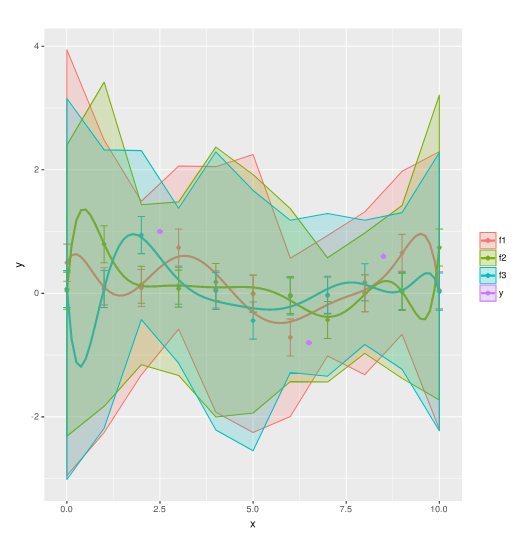
\includegraphics[width=.5\linewidth]{gpr_R_plot.png}
\end{figure}

Il codice sorgente completo di gpr\_R.pl si trova nel repository di 
Cplint on SWISH~\cite{gprRpl}.

\subsection{kalman\_filter\_R}
Il predicato \texttt{geom\_densities/7} disegna contemporanemente
due grafici in una sola figura grazie al pacchetto
\emph{gridExtra}~\cite{gridExtra}. Nella versione c3js, invece, tutti i dati 
sono rappresentati sullo stesso grafico.

Il grafico superiore si riferisce a un insieme di osservazioni e di stati, 
mentre quello inferiore rappresenta 4  distribuzioni di densità degli stati.

Il codice sorgente di questo esempio si trova nel repository~\cite{kalmanFilterRpl}.

\subsection{seven\_scientists\_R}
Il predicato \texttt{geom\_bar/1}  genera un diagramma a barre 
della media del valore dei campioni per ogni misurazione. Poichè 
abbiamo 7 elementi fissi sulle ascisse dobbiamo usare \texttt{numlist(1,7,X)}, 
una lista da 7 elementi e \texttt{breaks=seq(0,7,1)} per evidenziare i 7 
punti sul grafico. Si è inoltre usato \texttt{breaks=seq(0,max(df\$val),2)} 
per imitare il comportamento della versione c3js.

Il codice sorgente si trova nel repository di Cplint On 
SWISH~\cite{sevenScientistsRpl}.



%%%%
%%%%
%%%%
%%%%


\chapter{Conclusioni}

[TODO]

%%%%
%%%%
%%%%
%%%%

[TODO: Check all bibliography: page number, authors, references, etc...]

\printbibliography

\end{document}
